\documentclass[14pt,a4paper]{extarticle}


\setlength{\topmargin}{-2cm}
\setlength{\oddsidemargin}{0cm}
\setlength{\textheight}{24cm}
\setlength{\textwidth}{16cm}



\usepackage{graphicx}
\usepackage{listings}

\usepackage{amsmath}
\usepackage{algorithm}
\usepackage[noend]{algpseudocode}

%Use helvetica as sans serif
\usepackage{helvet}



\begin{document}


\title{LINE FOLLOWING BEHAVIOR FOR AN AUTONOMOUS MOBILE ROBOT USING ARTIFICIAL NEURAL NETWORKS}

\author{Manash Kumar Mandal\\ 1203043 \\ Department of Electrical \& Electronic Engineering \\ Khulna University of Engineering \& Technology}

\date{}

\maketitle
	

\tableofcontents

\newpage


\begin{abstract}

In order to achieve tasks by the mobile robots, these robotic systems must have been intelligent and should decide their own action. To guarantee the autonomy and the intelligence for line following behavior, it is necessary to use the techniques of artificial intelligence like the artificial neural networks. This project report presents an approach for line following task by an autonomous mobile robot using a single layer neural network. The proposed controller is used for following any line on a plain surface with different width. This controller can also be upgraded to determine the value of $k_{p}$ and $k_{d}$ and make the autonomous line following a $PD$ controller based. The results acquired from Neural Network simulation and implementation on the robot are shown and discussed.

\end{abstract}

\providecommand{\keywords}[1]{\textbf{\textit{Keywords-}} #1}

\keywords{Feedforward Neural Network, Artificial Intelligence, Robotics, Stochastic Gradient Descent, Proportional Derivative Controller}

\section{Introduction}

The line follower is a self operating robot that detects and follows a line that is drawn on the floor. The path consists of a black line on a white surface (or it may be reverse of that). The control system used must sense a line and maneuver the robot to stay on course, while constantly correcting the wrong moves using feedback mechanism, thus forming a simple yet effective closed loop system. The robot is designed to follow very tight curves. 

In this project, the conventional control system is being replaced by artificial neural network. 

	\subsection{Line detection mechanism}
	Line can be detected by either using Infra-red (IR) sensors, Light Dependent Resistor (LDR) or by a camera with line detection algorithms. Line tracking is a very important notion in the world of robotics as it give to the robot a precise, error-less and easy to implement navigation scheme. 
	
		\paragraph{Detecting line using IR}
		To detect line using IR, a threshold value must be measured. IR sensor gives different reading on different colored surface. Both values from IR on white line and IR on black line must be recorded before sensing the line.
		
		
		\begin{figure}[!h]
				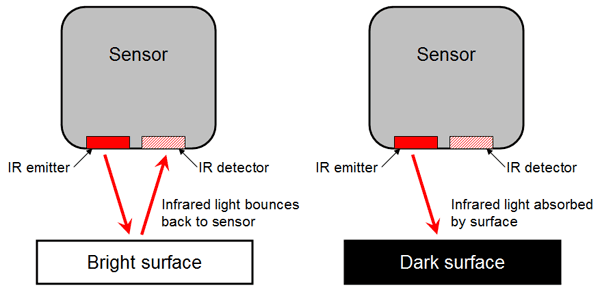
\includegraphics[width=\textwidth]{ir_line.png}
				\caption{Detecting line using IR sensor}
				\label{fig:detect_line_ir}
		\end{figure}
		
		\paragraph{Detecting line using LDR}
		To detect line using LDR same procedure from IR can be used. Since reflected line intensity depends on the reflecting surface. If the color of the surface is white, maximum light is reflected. If it is black then minimum light is reflected. Reflected light has different intensity based on the color of the surface it is being reflected from. So, nearest colors can be differentiated using LDR sensors. 
		
		\begin{figure}[!h]
			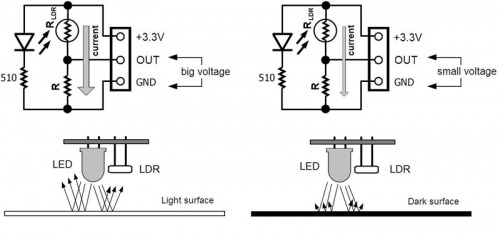
\includegraphics[width=\textwidth]{ldr_line.jpg}
			\caption{Detecting line using LDR sensor}
			\label{fig:detect_line_ldr}
		\end{figure}
			\subsection{Algorithm for detecting line}
		\begin{algorithm}
		\caption{Line Detecting Algorithm}\label{linetracker}
		\begin{algorithmic}[1]
		\Procedure{detectLine}{}
		
		\State $irPin \gets \text{ir receiver pin}$
		\State $irReading \gets \text {analog reading from ir receiver} $
		\State $threshold \gets \text {threshold value for differentiate betweeen white and black line} $
		\State $irDigitalReading \gets \text {converts analog into binary format} $
		
		\State $ irReading \gets \text{reading from irPin}$		
		\If {$irReading > \textit{threshold}$}
		\State $irDigitalReading \gets 1$
		\Else 
		\State $irDigitalReading \gets 0$
		\EndIf
		\EndProcedure
		\end{algorithmic}
		\end{algorithm}
		


	\subsection{Conventional line following mechanism}
	
	Conventional line following robots follow lines on a surface based on either predefined conditions or line patterns. 
	

	\subsection{Importance of the project}
	
	Robotics technology is emerging at a rapid pace, offering new possibilities for automating tasks in many challenging applications, especially in autonomous self driving vehicles. A lot of parameters and conditions and other necessary things are needed to be considered to build a complete autonomous self driving vehicles, yet making the vehicle to learn to follow the line of the path is one of the basic building blocks to build a complete autonomous self driving vehicles. The main objective of the project is to train a network and apply it on a autonomous line following prototype which can navigate autonomously at any line consisting of any width. 


\end{document}